\documentclass[11pt,letterpaper]{article}
\usepackage{amssymb,amsmath}
\usepackage{mathrsfs}
\usepackage{epsfig}
\usepackage{anysize}
\usepackage{verbatim}
\usepackage{minted} %% Código
\usepackage[utf8]{inputenc}
\usepackage[spanish]{babel}
\usepackage{listings}
\usepackage{tikz} %% Para dibujar una lista simplemente ligada
\usetikzlibrary{calc,shapes.multipart,chains,arrows, babel}
\usepackage{forest}

%% Cambiar "listing" por "listado"
\renewcommand\listingscaption{Listado}
\renewcommand{\lstlistingname}{Listado}


\title{Implementación de Árboles Patricia en Coq}
\author{Víctor Zamora Gutiérrez}
\date{\today}
\begin{document}
\maketitle
\thispagestyle{empty}
\begin{abstract}
  \noindent La meta de este trabajo fue realizar una implementación de árboles Patricia en Coq. Para esta implementación, era deseable demostrar que las operaciones principales funcionaban; con esto nos referimos a las operaciones de inserción y unión de árboles. La meta se logró de manera satisfactoria para la operación de inserción. Para la de unión, hubieron algunos problemas que evitaron que demostráramos propiedades sobre ella, pero al menos se demostró que la función utiliza recursión bien fundada.
\end{abstract}
\section{Introducción}
\noindent Los Árboles Patricia\cite{} son estructuras de datos que funcionan como diccionarios con llaves enteras. Son atractivos debido a la sencillez con la que se implementan en lenguajes funcionales y debido a su eficiencia. La idea básica es que se tiene un árbol en el que el $0$ representa ``izquierda'' y el $1$ representa ``derecha''. Por ejemplo, en el árbol de la figura~\ref{fig:Pat}, el elemento $y$ tiene llave $4$, pues $4=100$ y para llegar a $y$ tenemos que tomar el camino izquierda-izquierda-derecha (leyendo el número de adelante hacia atrás). Como podemos notar, los elementos siempre estarán en hojas de los árboles.

\begin{figure}[h]
\label{fig:Pat}
\caption{Figura obtenida en \cite{}}
\centering
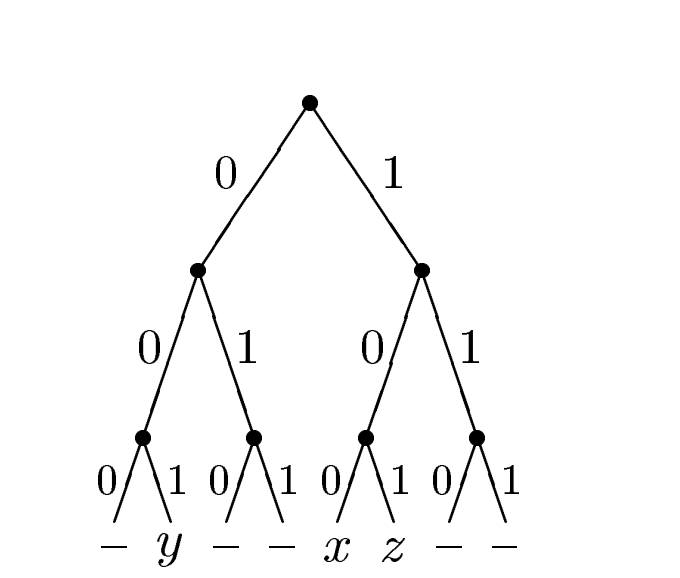
\includegraphics[ width=0.5\textwidth]{img/pat1}
\end{figure}

Por supuesto, si los árboles Patricia estuvieran implementados como el de la figura~\ref{fig:Pat}, no serían muy útiles, pues las búsquedas tomarían tiempo lineal sobre el tamaño de las llaves, lo cual no es muy óptimo. Por esto, de esta idea básica se obtienen varias optimizaciones para crear una estructura de datos eficiente, de las cuales hablaremos más adelante.

En este trabajo se decidió hacer una implementación de árboles Patricia en Coq. Se comenzó desde lo más básico, que son los tries binarios (estructuras de la figura~\ref{fig:Pat}) hasta llegar a la estructura final. Para la estructura final, se implementaron las operaciones de búsqueda, inserción y unión, de las cuales también hablaremos más adelante. Además se verificó el funcionamiento de la inserción con respecto a búsquedas. Para la unión no se verificó nada debido a la forma en la que tuvo que definirse; sin embargo se logró definir a pesar de que utiliza recursión distinta a la que se trabajó con Coq a lo largo del semestre.

\section{Estructura del Proyecto}
\noindent El proyecto está dividido en dos tipos de archivos: de definiciones y de proposiciones. Los archivos de definiciones son:
\begin{itemize}
  \item 
\end{itemize}

\section{Herramientas}

\noindent Para el desarrollo del proyecto, utilizamos algunas bibliotecas auxiliares de Coq. La más importante de estas fue la biblioteca \texttt{BinNat}\cite{} que define a los números naturales en binario. Esta biblioteca se usó para definir las llaves y la estructura general de los árboles. Además de esta, utilizamos las siguientes bibliotecas:
\begin{itemize}
\item \texttt{BinPos} - Para enteros positivos binarios (naturales sin cero).
\item \texttt{Lia} - Para demostrar propiedades de operaciones aritméticas.
\item \texttt{Bool.Bool} - Para propiedades sobre el tipo \texttt{Bool} de Coq.
\end{itemize}

\section{Desarrollo}

\subsection{Tries binarios}

\noindent Decidimos basarnos completamente en\cite{} para el desarrollo del proyecto. Esto implicó una optimización gradual del trie binario hasta llegar a árboles Patricia.

El trie binario es la estructura de datos de la figura~\ref{fig:Pat}. Básicamente es un árbol binario en el que cada arista está etiquetada con $0$ o $1$, dependiendo de si es arista izquierda o derecha. Los nodos internos no contienen ninguna información; son las hojas quienes contienen a los elementos del árbol. Nuestra definición del trie binario se encuentra en el listado~\ref{lst:trieBin}.

\begin{listing}[H]
  \inputminted{coq}{src/trie.v}
  \caption{Definición de trie binario}
  \label{lst:trieBin}
\end{listing}

La búsqueda en trie binario es sencilla. Para buscar una llave $x$ simplemente vemos si es par o impar. Si es par, buscamos por el lado izquierdo y si es impar buscamos por el derecho. Dividimos la llave entre dos y continuamos el proceso hasta llegar a una hoja. La función de búsqueda está en el listado~\ref{lst:lookup}.

\begin{listing}[H]
  \inputminted{coq}{src/lookup.v}
  \caption{Búsqueda en un trie binario}
  \label{lst:lookup}
\end{listing}


\subsection{Primera Optimización}
\noindent La primera optimización que se hace para los tries binarios es colapsar a dos subárboles vacíos en un solo árbol. Esto para decrementar el tamaño del árbol. Dicha optimización se logra por medio de un \textit{constructor inteligente}. La idea de los constructores inteligentes es que en lugar de utilizar el constructor \texttt{trie} del listado~\ref{lst:trieBin}, utilizaremos únicamente el constructor inteligente para construir nuestros árboles. El constructor inteligente se enecuentra en el listado~\ref{lst:smart1}.

\begin{listing}[H]
  \inputminted{coq}{src/smart1.v}
  \caption{Primera optimización de los tries binarios}
  \label{lst:smart1}
\end{listing}

\subsection{Segunda Optimización}
\noindent La segunda optimización sale de la siguiente consideración: supongamos que tenemos un árbol cuyo único elemento es una hoja y el resto de sus subárboles son vacíos. En la figura~\ref{fig:arbol_chafa} podemos ver un árbol así. Este árbol tiene un solo elemento; sin embargo, tenemos que recorrerlo todo para encontrar este elemento. Esto no tiene mucho sentido, y de aquí surge la idea de colapsar este tipo de árboles en un solo nodo. Para lograr esto, se usó la optimización del listado~\ref{lst:opt2}. Este listado contiene otro constructor inteligente que, al encontrar una hoja junto a un árbol vacío, colapsa el árbol vacío con la hoja.

\begin{figure}[h]
  \caption{Árbol con una sola hoja}
  \label{fig:arbol_chafa}
   \centering
  \begin{tikzpicture}
    \tikzstyle{every child node}=[circle,draw]
    \node(Root)[circle, draw]{}
    child[missing]{}
    child{node[circle,draw]{}
      child[missing]{}
      child{node[circle,draw]{}
        child[missing]{}
        child{node[circle,draw]{$n$} edge from parent node[right,draw=none] {$1$}}
        edge from parent node[right,draw=none] {$1$}
      }
      edge from parent node[right,draw=none] {$1$}
    };
  \end{tikzpicture}
\end{figure}

\begin{listing}[H]
  \inputminted{coq}{src/smart2.v}
  \caption{Segunda optimización de los tries binarios}
  \label{lst:opt2}
\end{listing}

Para que esta optimización funcionara, tuvimos que modificar la estructura de árbol para que las hojas guardaran un prefijo de su llave. La nueva estructura de árbol está en el listado~\ref{lst:prefix}.

\begin{listing}[H]
  \inputminted{coq}{src/prefix.v}
  \caption{Árboles cuyas hojas guardan una llave}
  \label{lst:prefix}
\end{listing}

Observemos que los prefijos que guardan las hojas son de tipo \texttt{N}. Este es el tipo para números binarios en Coq.

Después de realizar esta optimización, hay que modificar ligeramente la función de búsqueda para que al llegar a una hoja, revise que el prefijo de la hoja sea igual al elemento que busca.

\subsection{Tercera optimización}

\noindent Una alternativa a la optimización anterior es que en lugar de que las hojas guarden un prefijo de su llave, guarden la llave completa. Así, en la función de búsqueda ya no tenemos que descartar bits (o equivalentemente, dividir). Para que esto funcione, es necesario que los nodos guarden el bit sobre el que se dividen. Lo que esto quiere decir es que cada nodo guarda su profundidad, y así la función de búsqueda solo tiene que revisar el bit correspondiente a la profundidad del nodo.

Como guardar la profundidad complica los cálculos de buscar el bit correspondiente, en la práctica lo que se hace es guardar un entero binario con un solo bit prendido, y revisar dicho bit en la llave buscada.

Para esto, definimos la nueva estructura dada por el listado~\ref{lst:trie3}. La nueva función de búsqueda se encuentra en el listado~\ref{lst:lookup3}. La función \texttt{zeroBit} nos dice si el bit prendido de \texttt{m} está apagado en \texttt{key}. Podemos verla en el listado~\ref{lst:zeroBit}.

\begin{listing}[H]
  \inputminted{coq}{src/trie3.v}
  \caption{Estructura de datos definida de acuerdo a la nueva optimización}
  \label{lst:trie3}
\end{listing}

\begin{listing}[H]
  \inputminted{coq}{src/lookup3.v}
  \caption{Nueva función de búsqueda}
  \label{lst:lookup3}
\end{listing}

\begin{listing}[H]
  \inputminted{coq}{src/zeroBit.v}
  \caption{Función que revisa si un bit está apagado}
  \label{lst:zeroBit}
\end{listing}

\nocite{*}
 \bibliographystyle{IEEEtran}
 \bibliography{Proyecto}

\end{document}
